\documentclass{article}
\usepackage{amsmath}
\usepackage{pgfplots}
\usepackage{float}
\pgfplotsset{compat=1.17}
\begin{document}

\title{Electricity and Magnetism - Lecture 9 Notes}
\author{Joshua Clement}
\maketitle

\section*{Electric Potential (Voltage Relative to Infinity)}
\begin{itemize}
    \item \textbf{Electric Potential} (\(V\)): The potential energy per unit charge due to the presence of other charges.
    \item \textbf{Potential at Infinity}: Defined as zero by convention, consistent with electric potential energy being zero for two charges infinitely separated.
    \item \textbf{Potential Due to One Particle}:
    \[
    V(r) = \frac{1}{4 \pi \epsilon_0} \frac{q}{r}
    \]
    where \(q\) is the charge and \(r\) is the distance from the charge.
\end{itemize}

\begin{figure}[h!]
    \centering
    % Start first minipage for Positive Charge
    \begin{minipage}{0.35\textwidth}
        \centering
        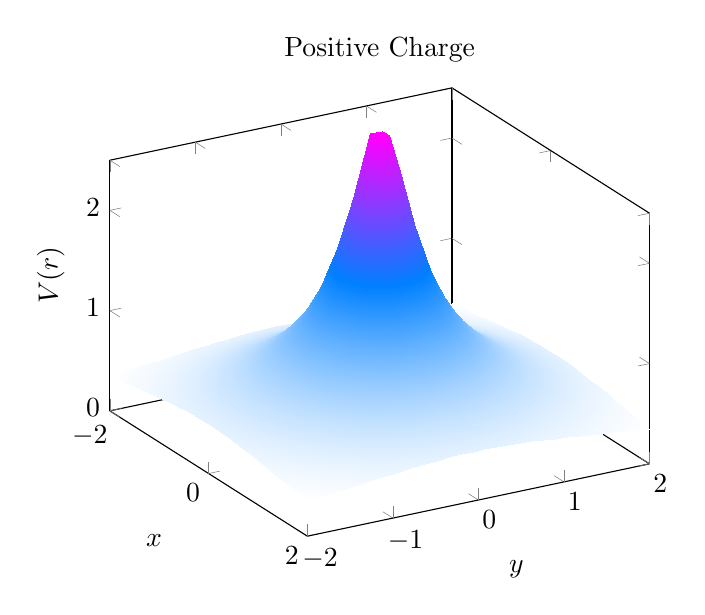
\begin{tikzpicture}
            \begin{axis}[
                view={60}{30},
                xlabel={$x$},
                ylabel={$y$},
                zlabel={$V(r)$},
                domain=-2:2,
                y domain=-2:2,
                colormap/cool,
                samples=30,
                samples y=30,
                zmax=2.5,
                zmin=0,
                mesh/ordering=y varies,
                title={Positive Charge}
            ]
                \addplot3[
                    surf,
                    shader=interp,
                    domain=-2:2,
                    y domain=-2:2,
                    ]
                    {1/sqrt(x^2 + y^2 + 0.1)};
            \end{axis}
        \end{tikzpicture}
    \end{minipage}%
    \hspace{0.29\textwidth} % Space between the two plots
    % Start second minipage for Negative Charge
    \begin{minipage}{0.35\textwidth}
        \centering
        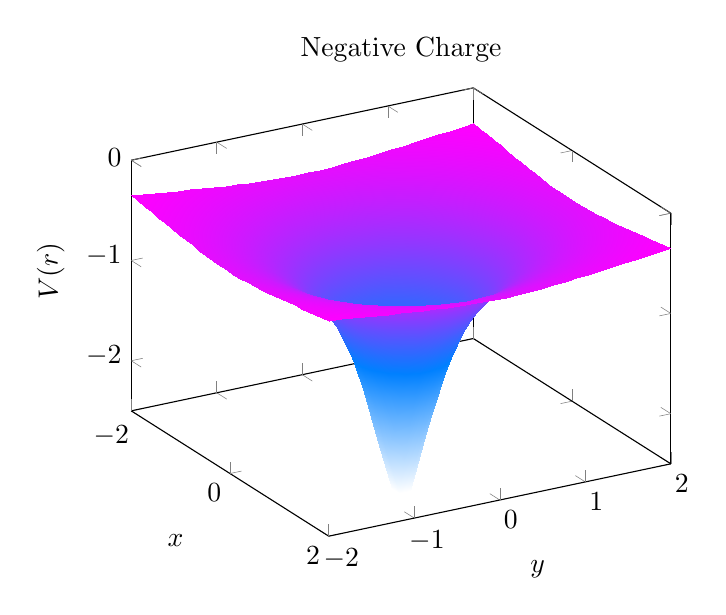
\begin{tikzpicture}
            \begin{axis}[
                view={60}{30},
                xlabel={$x$},
                ylabel={$y$},
                zlabel={$V(r)$},
                domain=-2:2,
                y domain=-2:2,
                colormap/cool,
                samples=30,
                samples y=30,
                zmax=0,
                zmin=-2.5,
                mesh/ordering=y varies,
                title={Negative Charge}
            ]
                \addplot3[
                    surf,
                    shader=interp,
                    domain=-2:2,
                    y domain=-2:2,
                    ]
                    {-1/sqrt(x^2 + y^2 + 0.1)};
            \end{axis}
        \end{tikzpicture}
    \end{minipage}

    \caption{Electric field always points in the direction of steepest descent of V (steepest slope) and its magnitude is the slope.}
    \label{fig:potential_scalar_field}
\end{figure}
\section*{Potential Difference and Electric Field}
\begin{itemize}
    \item \textbf{Potential Difference} (\(\Delta V\)): Difference in electric potential between two points.
    \[
    \Delta V = V_f - V_i = -\int_i^f \vec{E} \cdot d\vec{l}
    \]
    \item \textbf{Uniform Electric Field} (\(E \parallel x\)):
    \[
    \Delta V = -E \Delta x
    \]
    \item \textbf{Non-Uniform Electric Field}: The potential difference is obtained using the line integral of the electric field along the path.
\end{itemize}

\section*{Path Independence of Potential Difference}
\begin{itemize}
    \item \textbf{Path Independence}: The potential difference between two points does not depend on the path taken, only on the endpoints.
    \item \textbf{Round Trip Path}: For a complete loop, the potential difference is zero (\(\Delta V = 0\)).
    \item \textbf{Example}: Moving from point A to B and back results in \(\Delta V = 0\), similar to changes in height for a round trip up and down a mountain.
\end{itemize}

\section*{Electric Potential and Electric Field}
\begin{itemize}
    \item \textbf{Electric Field Direction}: The electric field points in the direction where the potential decreases most rapidly.
    \item \textbf{Relation Between Potential and Field}:
    \[
    E_x = -\frac{\partial V}{\partial x}, \quad E_y = -\frac{\partial V}{\partial y}, \quad E_z = -\frac{\partial V}{\partial z}
    \]
    \item \textbf{Gradient}: The electric field is the negative gradient of the electric potential:
    \[
    \vec{E} = -\nabla V
    \]
\end{itemize}

\section*{Electric Potential of a Uniformly Charged Shell}
\begin{itemize}
    \item \textbf{Outside the Shell} (\(r > R\)):
    \[
    V(r) = \frac{1}{4 \pi \epsilon_0} \frac{Q}{r}
    \]
    where \(Q\) is the total charge and \(R\) is the radius of the shell.
    \item \textbf{Inside the Shell} (\(r \leq R\)):
    \[
    V(r) = \frac{1}{4 \pi \epsilon_0} \frac{Q}{R}
    \]
    The potential inside is constant.
\end{itemize}

\section*{Calculating Electric Field from Potential}
\begin{itemize}
    \item \textbf{Direction of Electric Field}: Points in the direction of the steepest descent of the potential (\(V\)).
    \item \textbf{Magnitude of Electric Field}: Related to the slope of the potential function.
    \item \textbf{Example}:
    \begin{itemize}
        \item \textbf{Positive Charge}: Electric potential decreases with increasing distance, and the field points away from the charge.
        \item \textbf{Negative Charge}: Electric potential increases (becomes less negative) with increasing distance, and the field points toward the charge.
    \end{itemize}
\end{itemize}


\end{document}